\documentclass[a4paper]{article}
\usepackage[left=2cm, right=2cm, top=2cm]{geometry}
\usepackage{tikz}
\usepackage{algorithm}
\usepackage{graphicx}
\usepackage{float}
\usepackage{listings}

\def\code#1{\texttt{#1}}

\lstset{
frame=single
}

\author{Kevin Mambu}
\title{UE-VLSI2 TP : Cadence RTL Compiler \\ Kévin Mambu}
\begin{document}
\maketitle

\section{Set the environment}

\lstinputlisting[language=bash]{../set_env.sh}


\section{Load the libraries}

{\it n.b: all the libraries are located at} \code{/users/enseig/tuna/ue-vlsi2/techno}.

Two types of cell libraries are available:
\code{\_Best.lib} and \code{\_Worst.lib}. The difference between these libraries
lies in the timing arcs of their cells : while the Best Library contains Best-Case timings,
the Worst Library contains the Worst-Case equivalents. Each timing arcs are estimated via
different PVT parameters (\textbf{Process - Voltage - Temperature}). These parameters an be
found in the headers of each library.

\lstinputlisting{cmos_120nm_core_Worst_header.txt}
\begin{center}
  \it{PVT specifications for cmos\_120nm\_core\_Worst}
\end{center}

\newpage

\lstinputlisting{cmos_120nm_core_Best_header.txt}
\begin{center}
  \it{PVT specifications for cmos\_120nm\_core\_Best}
\end{center}

In order to synthesize the RTL description, we will use cmos\_120nm\_core\_Worst.lib.
This library contains all the generic cells we will need, and with Worst-Case timings
in order to thoroughly stress the longest combinational paths.

A practical example of difference in timing arcs between this library and its \_Best
equivalent can be seen when evaluating the ND2AHS cell, a "2 Input NAND w\/ A Input
Inverted and 1x Drive".

\begin{center}
  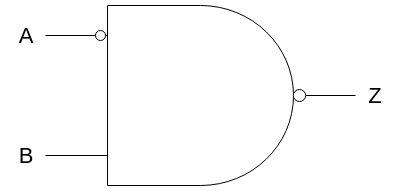
\includegraphics[width=10cm]{./nd2ahs.png} \newline
  \it{Gate-level schematic of the ND2AHS cell}
\end{center}
% TODO : mettre un comparatif WC/BC
%        demander à l'homme-sirène s'il faut faire le schéma symbolique de la
%        cellule?
\section{Load the design}

\section{Elaborate}

The eaboration process does not differ from the Synthesis per se. The elaboration step
is the conversion of the RTL description to a model where every instance object (signal,
process, arrays, etc) is converted into a component (adder, multiplexer, register, etc).
This step is part of the Synthesis process.

\section{Check design}

\section{Synthesis}

\section{Reset}

\section{Reporting}


\end{document}
